\section{12 Sept 23 - Notes: Dynamical Systems and Phase
Space}\label{sept-23---notes-dynamical-systems-and-phase-space}

Dynamical systems is a branch of mathematics that seeks to investigate
the time dependence of a system and characterize the families of
trajectories that the system can have. We don't often solve the system
for a given set of initial conditions in dynamical systems work.
Instead, we want to \textbf{uncover the families of possible solutions}
for a system to see what kinds of things it \emph{can} do. An excellent
book on this subject that we will draw from is Strogatz's book on
Nonlinear Dynamics \{cite\}\texttt{strogatz2018nonlinear}; I highly
recommend you find a copy for yourself.

\subsection{Geometric Thinking and Phase
Portraits}\label{geometric-thinking-and-phase-portraits}

One of the first things we will use to investigate systems from a
dynamical systems perspective is the
\href{https://en.wikipedia.org/wiki/Phase_portrait}{phase portrait},
where we will plot the velocity against the position. We can use the
phase portrait to tell us what families of solutions we might expect to
see.

\emph{Phase portraits are quite useful for second order differential
equations (or any two-dimensional system) because we frequently use and
interpret 2D graphs.} Notice that we focused on ``2nd order differential
equations'' not ``linear 2nd order.'' That is because, as we will see,
\textbf{phase portraits are particularly useful for nonlinear 2nd order
differential equations.}

\subsection{Lecture Video}\label{lecture-video}

We will go into the details of how to construct and develop phase
portraits in class. This video from
\href{https://www.me.washington.edu/facultyfinder/steve-brunton}{Steve
Brunton} is a good overview of the process. It's quite detailed and
takes a mathematical perspective, so don't worry if you don't understand
everything in the video. We have plenty of time to investigate how this
works in practice.

\href{https://inv.tux.pizza/watch?v=vBwyD4JJlSs}{\pandocbounded{\includegraphics[keepaspectratio]{https://markdown-videos-api.jorgenkh.no/youtube/vBwyD4JJlSs?width=720&height=405}}}

\begin{itemize}
\tightlist
\item
  Non-Commercial Link: \url{https://inv.tux.pizza/watch?v=vBwyD4JJlSs}
\item
  Commercial Link: \url{https://youtube.com/watch?v=vBwyD4JJlSs}
\end{itemize}

\begin{Shaded}
\begin{Highlighting}[]
\ImportTok{import}\NormalTok{ numpy }\ImportTok{as}\NormalTok{ np}
\ImportTok{import}\NormalTok{ matplotlib.pyplot }\ImportTok{as}\NormalTok{ plt}
\end{Highlighting}
\end{Shaded}

\subsection{The Phase Portrait of the
SHO}\label{the-phase-portrait-of-the-sho}

To get this started, let's develop the phase portrait of the SHO. Recall
that we separated the second order ODE into two first order ODEs, one
for \(x\) and one for \(v_x\),

\[\dot{x} = v_x\] \[\dot{v}_x=-\omega^2x\]

We then map out the phase space with the following conceptual
interpretation:

\begin{itemize}
\tightlist
\item
  Phase space is a space in which all possible states of the system can
  be shown

  \begin{itemize}
  \tightlist
  \item
    a state is a collection of conditions of the state (it's known
    position and velocity in our case)
  \end{itemize}
\item
  Each state is a unique point in phase space

  \begin{itemize}
  \tightlist
  \item
    Think about ordered Cartesian pairs, there's a pair of numbers for
    every point in a 2D space
  \end{itemize}
\item
  Remember that knowing \(x_0\) and \(v_{x,0}\) means we can know
  \(x(t)\) for all time (for that one trajectory/particular solution)
  given a linear ODE
\end{itemize}

We map the differential equation to the following conceptual
interpretation: \textbf{How the state changes depends on location in
phase space.} We can understand this as the time derivative for \(x\)
and \(v_x\) change throughout the space.

For our 2D SHO case we are saying that how \(x\) and \(v_x\) change is
proportional to the position in space:

\[\langle \dot{x}, \dot{v}_x \rangle = \langle v_x, -\omega^2 x\rangle\]

The process is:

\begin{enumerate}
\def\labelenumi{\arabic{enumi}.}
\tightlist
\item
  Determine the location(s) of interest (i.e., \(x\), \(v_x\))
\item
  Compute the change in those quantities at the location (i.e.,
  calculate \(\dot{x}\) and \(\dot{v}_x\) using our prescribed 1st order
  ODEs above)
\item
  At a given point (\(x_0\), \(v_{x,0}\)), create an arrow the indicates
  the direction and magnitude of the changes to \(x\) and \(v_x\) at
  that location.

  \begin{itemize}
  \tightlist
  \item
    That arrow represents the local flow of the system at that point
  \end{itemize}
\item
  Repeat for all points of interest
\item
  Plot arrows to demonstrate flow of the solutions in phase space
\end{enumerate}

\subsubsection{Let's focus on axes
first}\label{lets-focus-on-axes-first}

We talked about how we can look at the axes (\(x=0\) and \(v_x =0\)) to
help get a sense of the flow in phase space. Below, we have some code
that does this in two parts: 1. We created a function to produce arrows
of the right length given a line of points 2. We call that function for
each axis and for a line at a diagonal

\subsubsection{Questions to consider.}\label{questions-to-consider.}

\begin{enumerate}
\def\labelenumi{\arabic{enumi}.}
\tightlist
\item
  Review the phase portraits below. How are they constructed?

  \begin{itemize}
  \tightlist
  \item
    Work to identify which components of the code look familiar and
    which you have more questions about
  \end{itemize}
\item
  Try to make a fourth plot that looks at the other diagonal line that
  runs at a 45 degree angle to each axes
\end{enumerate}

\textbf{You should be able to explain what the code is doing.} We
avoided using Numpy's
\href{https://numpy.org/doc/stable/reference/generated/numpy.meshgrid.html}{meshgrid}
here to make this a smaller bit of code.

\subsubsection{PlotPhaseSpaceAxesSHO}\label{plotphasespaceaxessho}

This function is computing the arrows for a given line of points in
phase space. Send it a line of points in two arrays (one for \(x\) and
one for \(v_x\)) and it plots the resulting arrows. The code is
documented below with comments and then used several times.

\begin{Shaded}
\begin{Highlighting}[]
\KeywordTok{def}\NormalTok{ PlotPhaseSpaceAxesSHO(x, vx, N}\OperatorTok{=}\DecValTok{20}\NormalTok{):}
    \CommentTok{"""Takes two one{-}dimensional arrays}
\CommentTok{    and computes the resulting arrow to}
\CommentTok{    represent the flow of the system in }
\CommentTok{    phase space. This code is specifically}
\CommentTok{    designed for the SHO with omega=1"""}

    \CommentTok{\#\# Map the points to the arrows using the }
    \CommentTok{\#\# 1st order ODEs for the SHO}
    \CommentTok{\#\# Returns two arrays of the same length}
    \CommentTok{\#\# as the inputs}
\NormalTok{    xdot, vxdot }\OperatorTok{=}\NormalTok{ vx, }\OperatorTok{{-}}\DecValTok{1}\OperatorTok{*}\NormalTok{x}

    \CommentTok{\#\# Create a figure with a known size}
\NormalTok{    plt.figure(figsize}\OperatorTok{=}\NormalTok{(}\DecValTok{10}\NormalTok{,}\DecValTok{8}\NormalTok{))}

    \CommentTok{\#\# Go through all the arrays we created to plot the arrows}
    \CommentTok{\#\# Syntax for arrow is:}
    \CommentTok{\#\# arrow(xpos, ypos, xchange, ychange, other\_parameters)}
    \ControlFlowTok{for}\NormalTok{ i }\KeywordTok{in}\NormalTok{ np.arange(N):}
    
\NormalTok{        plt.arrow(x[i], vx[i], xdot[i], vxdot[i], }
\NormalTok{                  head\_width}\OperatorTok{=}\FloatTok{0.2}\NormalTok{, }
\NormalTok{                  head\_length}\OperatorTok{=}\FloatTok{0.2}\NormalTok{)}
\NormalTok{        plt.xlabel(}\StringTok{\textquotesingle{}$x$\textquotesingle{}}\NormalTok{)}
\NormalTok{        plt.ylabel(}\StringTok{\textquotesingle{}$v\_x$\textquotesingle{}}\NormalTok{)}
        
\NormalTok{    plt.grid()}
\end{Highlighting}
\end{Shaded}

\subsubsection{Plotting along the vx
axis}\label{plotting-along-the-vx-axis}

\begin{Shaded}
\begin{Highlighting}[]
\CommentTok{\#\# Plotting along the vx axis}
\NormalTok{N }\OperatorTok{=} \DecValTok{20}

\NormalTok{x }\OperatorTok{=}\NormalTok{ np.zeros(N)}
\NormalTok{vx }\OperatorTok{=}\NormalTok{ np.linspace(}\OperatorTok{{-}}\DecValTok{5}\NormalTok{,}\DecValTok{6}\NormalTok{,N)}

\NormalTok{PlotPhaseSpaceAxesSHO(x, vx, N)}
\end{Highlighting}
\end{Shaded}

\begin{figure}
\centering
\pandocbounded{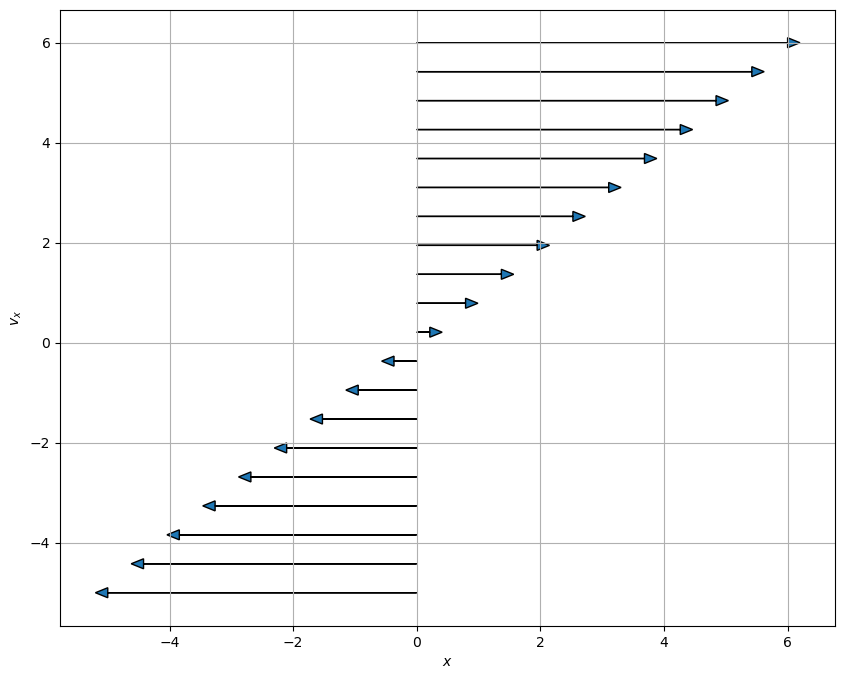
\includegraphics[keepaspectratio,alt={png}]{../images/notes-phase_space_notes-phase_space_tmp_6_0.png}}
\caption{png}
\end{figure}

\subsubsection{Plotting along the x
axis}\label{plotting-along-the-x-axis}

\begin{Shaded}
\begin{Highlighting}[]
\CommentTok{\#\# Plotting along the x axis}
\NormalTok{N }\OperatorTok{=} \DecValTok{20}

\NormalTok{x }\OperatorTok{=}\NormalTok{ np.linspace(}\OperatorTok{{-}}\DecValTok{5}\NormalTok{,}\DecValTok{6}\NormalTok{,N)}
\NormalTok{vx }\OperatorTok{=}\NormalTok{ np.zeros(N)}

\NormalTok{PlotPhaseSpaceAxesSHO(x, vx, N)}
\end{Highlighting}
\end{Shaded}

\begin{figure}
\centering
\pandocbounded{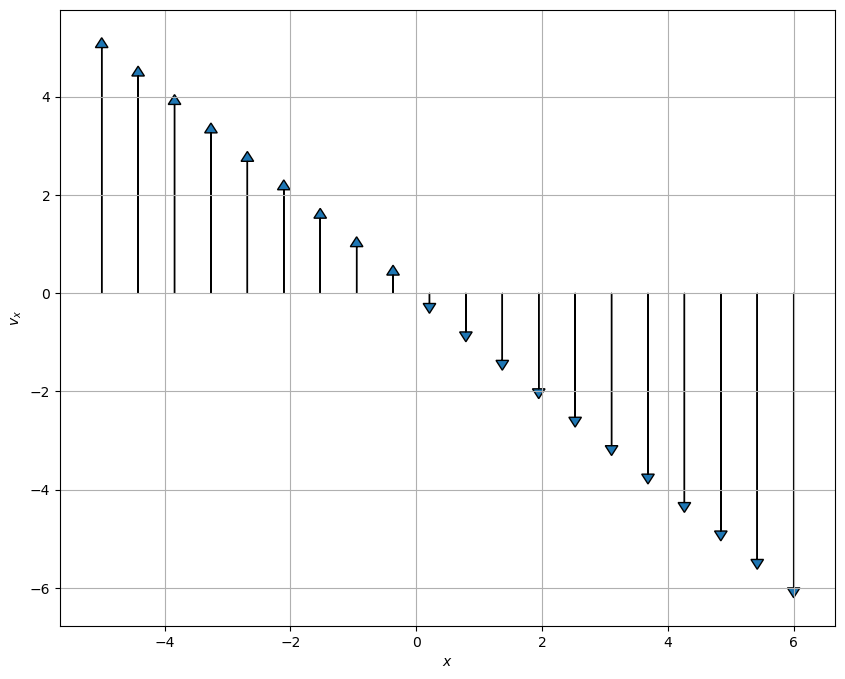
\includegraphics[keepaspectratio,alt={png}]{../images/notes-phase_space_notes-phase_space_tmp_8_0.png}}
\caption{png}
\end{figure}

\subsubsection{Plotting along the 45 degree line between the x and vx
axes}\label{plotting-along-the-45-degree-line-between-the-x-and-vx-axes}

\begin{Shaded}
\begin{Highlighting}[]
\CommentTok{\#\# Plotting along the 45 degree line between the x and vx axes}
\NormalTok{N }\OperatorTok{=} \DecValTok{20}

\NormalTok{x }\OperatorTok{=}\NormalTok{ np.linspace(}\OperatorTok{{-}}\DecValTok{5}\NormalTok{,}\DecValTok{6}\NormalTok{,N)}
\NormalTok{vx }\OperatorTok{=}\NormalTok{ np.linspace(}\OperatorTok{{-}}\DecValTok{5}\NormalTok{,}\DecValTok{6}\NormalTok{,N)}

\NormalTok{PlotPhaseSpaceAxesSHO(x, vx, N)}
\end{Highlighting}
\end{Shaded}

\begin{figure}
\centering
\pandocbounded{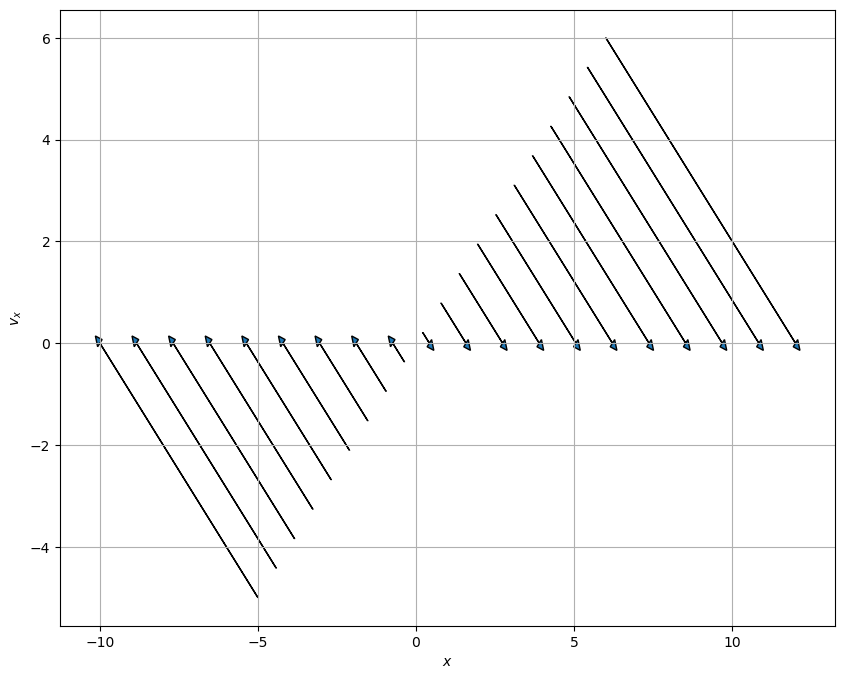
\includegraphics[keepaspectratio,alt={png}]{../images/notes-phase_space_notes-phase_space_tmp_10_0.png}}
\caption{png}
\end{figure}

\subsubsection{Make a Graph}\label{make-a-graph}

\textbf{✅ Do this}

\begin{enumerate}
\def\labelenumi{\arabic{enumi}.}
\tightlist
\item
  Make a fourth plot that looks at the other diagonal line that runs at
  a 45 degree angle to each axes
\end{enumerate}

\begin{Shaded}
\begin{Highlighting}[]
\CommentTok{\#\# Your code here}
\CommentTok{\#\# Plot the other 45 degree line}
\end{Highlighting}
\end{Shaded}

\subsection{Phase Portrait of the Simple Harmonic
Oscillator}\label{phase-portrait-of-the-simple-harmonic-oscillator}

Below, we have written code that makes a phase portrait from the simple
harmonic oscillator. It's written in terms of three functions that serve
three purposes that you might want to modify in your own work:

\begin{itemize}
\tightlist
\item
  \texttt{SHOPhasePortrait} is a function that simply returns the
  relationship between the locations in phase space and how the phase
  variables change at that location.
\item
  \texttt{ComputeSHOPhase} is a function that uses that relationship and
  computes the values of the changes at every location. It returns two
  arrays, which contain all those values.
\item
  \texttt{SHOTrajectory} is a function that takes a pair of points in
  space and computes the trajectory in phase space
\end{itemize}

By separating these ideas, we are illustrating the process for computing
these phase portraits: - Translate the \(N\)th order differential
equation to \(N\) 1st order (Done earlier in this case) - Put that into
a code so you can compute the value of the changes at a location
(\texttt{SHOPhasePotrait}) - Call that computation a bunch to compute it
at every location you want (\texttt{ComputeSHOPhase}) - investigate
specific trajectories in the space (\texttt{SHOTrajectory})

We can then call these functions can plots the results.

\begin{Shaded}
\begin{Highlighting}[]
\KeywordTok{def}\NormalTok{ SHOPhasePortrait(x, vx, omega):}
    \CommentTok{\textquotesingle{}\textquotesingle{}\textquotesingle{}SHOPhasePortrait returns the value of}
\CommentTok{    the change in the phase variables at a given location}
\CommentTok{    in phase space for the SHO model\textquotesingle{}\textquotesingle{}\textquotesingle{}}
    
\NormalTok{    xdot, vxdot }\OperatorTok{=}\NormalTok{ [vx, }\OperatorTok{{-}}\DecValTok{1}\OperatorTok{*}\NormalTok{omega}\OperatorTok{**}\DecValTok{2}\OperatorTok{*}\NormalTok{x] }\CommentTok{\#\# Specific to this problem}
    
    \ControlFlowTok{return}\NormalTok{ xdot, vxdot}
\end{Highlighting}
\end{Shaded}

\begin{Shaded}
\begin{Highlighting}[]
\KeywordTok{def}\NormalTok{ ComputeSHOPhase(X, VX, omega):}
    \CommentTok{\textquotesingle{}\textquotesingle{}\textquotesingle{}ComputeSHOPhase returns the changes in }
\CommentTok{    the phase variables across a grid of locations}
\CommentTok{    that are specified\textquotesingle{}\textquotesingle{}\textquotesingle{}}
    
    \CommentTok{\#\# Prep the arrays with zeros at the right size}
\NormalTok{    xdot, vxdot }\OperatorTok{=}\NormalTok{ np.zeros(X.shape), np.zeros(VX.shape)}

    \CommentTok{\#\# Set the limits of the loop based on how }
    \CommentTok{\#\# many points in the arrays we have}
\NormalTok{    Xlim, Ylim }\OperatorTok{=}\NormalTok{ X.shape}
    
    \CommentTok{\#\# Calculate the changes at each location and add them to the arrays}
    \ControlFlowTok{for}\NormalTok{ i }\KeywordTok{in} \BuiltInTok{range}\NormalTok{(Xlim):}
        \ControlFlowTok{for}\NormalTok{ j }\KeywordTok{in} \BuiltInTok{range}\NormalTok{(Ylim):}
\NormalTok{            xloc }\OperatorTok{=}\NormalTok{ X[i, j]}
\NormalTok{            yloc }\OperatorTok{=}\NormalTok{ VX[i, j]}
\NormalTok{            xdot[i,j], vxdot[i,j] }\OperatorTok{=}\NormalTok{ SHOPhasePortrait(xloc, yloc, omega)}
            
    \ControlFlowTok{return}\NormalTok{ xdot, vxdot}
\end{Highlighting}
\end{Shaded}

\begin{Shaded}
\begin{Highlighting}[]
\KeywordTok{def}\NormalTok{ SHOTrajectory(x0, vx0, omega, N}\OperatorTok{=}\DecValTok{100}\NormalTok{):}
    \CommentTok{\textquotesingle{}\textquotesingle{}\textquotesingle{}SHOTrajectory computes the phase space}
\CommentTok{    trjectory using the analytical forms of the}
\CommentTok{    solution. Note this sloppy analytical approach}
\CommentTok{    only works because the SHO is perfectly sinusoidal.\textquotesingle{}\textquotesingle{}\textquotesingle{}}
    
    \CommentTok{\#\# Only work with one period}
\NormalTok{    T }\OperatorTok{=} \DecValTok{2}\OperatorTok{*}\NormalTok{np.pi}\OperatorTok{/}\NormalTok{omega}
\NormalTok{    t }\OperatorTok{=}\NormalTok{ np.arange(}\DecValTok{0}\NormalTok{,T,T}\OperatorTok{/}\NormalTok{N)}
    
    \CommentTok{\#\# I derived this in general with Acos(wt+phi)}
    \CommentTok{\#\# It\textquotesingle{}s not in general a good approach}
    \CommentTok{\#\# because you are not guaranteed analytical }
    \CommentTok{\#\# closed form trajectories in phase space}
    
\NormalTok{    phi }\OperatorTok{=}\NormalTok{ np.arctan2(}\OperatorTok{{-}}\DecValTok{1}\OperatorTok{*}\NormalTok{vx0, omega}\OperatorTok{*}\NormalTok{x0) }\CommentTok{\#\# arctan({-}vxo/(omega*x0)) taken correctly for the quadrant}
\NormalTok{    A }\OperatorTok{=}\NormalTok{ x0}\OperatorTok{/}\NormalTok{np.cos(phi)}
\NormalTok{    x\_traj }\OperatorTok{=}\NormalTok{ A}\OperatorTok{*}\NormalTok{np.cos(omega}\OperatorTok{*}\NormalTok{t}\OperatorTok{+}\NormalTok{phi)}
\NormalTok{    v\_traj }\OperatorTok{=} \OperatorTok{{-}}\NormalTok{omega}\OperatorTok{*}\NormalTok{A}\OperatorTok{*}\NormalTok{np.sin(omega}\OperatorTok{*}\NormalTok{t}\OperatorTok{+}\NormalTok{phi)}
    
    \ControlFlowTok{return}\NormalTok{ x\_traj, v\_traj}
\end{Highlighting}
\end{Shaded}

\subsubsection{Putting the functions to
use}\label{putting-the-functions-to-use}

With these two functions, all we are left to do is specify the size of
the space and the grid points (that is where exactly we are computing
the changes). We use
\href{https://numpy.org/doc/stable/reference/generated/numpy.meshgrid.html}{meshgrid}
to make those arrays a set of Cartesian coordinates and then send that
to our functions.

We then plots the results.

\begin{Shaded}
\begin{Highlighting}[]
\CommentTok{\#\# Setting parameters and the phase space variables}

\NormalTok{omega }\OperatorTok{=} \DecValTok{1}
\NormalTok{x }\OperatorTok{=}\NormalTok{ np.linspace(}\OperatorTok{{-}}\FloatTok{10.0}\NormalTok{, }\FloatTok{10.0}\NormalTok{, }\DecValTok{20}\NormalTok{)}
\NormalTok{vx }\OperatorTok{=}\NormalTok{ np.linspace(}\OperatorTok{{-}}\FloatTok{10.0}\NormalTok{, }\FloatTok{10.0}\NormalTok{, }\DecValTok{20}\NormalTok{)}

\CommentTok{\#\# Get back pairs of coordinates for every point in the space}
\NormalTok{X, VX }\OperatorTok{=}\NormalTok{ np.meshgrid(x, vx)}

\CommentTok{\#\# Run our calculations}
\NormalTok{xdot, vxdot }\OperatorTok{=}\NormalTok{ ComputeSHOPhase(X, VX, omega)}

\NormalTok{x0 }\OperatorTok{=} \DecValTok{5}
\NormalTok{vx0 }\OperatorTok{=} \DecValTok{3}
\NormalTok{x\_traj, v\_traj }\OperatorTok{=}\NormalTok{ SHOTrajectory(x0, vx0, omega)}

\CommentTok{\#\# Plot. plot. plot.}
\NormalTok{ax }\OperatorTok{=}\NormalTok{ plt.figure(figsize}\OperatorTok{=}\NormalTok{(}\DecValTok{10}\NormalTok{,}\DecValTok{6}\NormalTok{))}
\NormalTok{Q }\OperatorTok{=}\NormalTok{ plt.quiver(X, VX, xdot, vxdot, color}\OperatorTok{=}\StringTok{\textquotesingle{}k\textquotesingle{}}\NormalTok{)}

\CommentTok{\#\# Plot trajectory and the starting location}
\NormalTok{plt.plot(x\_traj,v\_traj)}
\NormalTok{plt.plot(x0, vx0, }\StringTok{\textquotesingle{}r*\textquotesingle{}}\NormalTok{, markersize}\OperatorTok{=}\DecValTok{10}\NormalTok{)}

\NormalTok{plt.xlabel(}\StringTok{\textquotesingle{}$x$\textquotesingle{}}\NormalTok{)}
\NormalTok{plt.ylabel(}\StringTok{\textquotesingle{}$v\_x$\textquotesingle{}}\NormalTok{)}
\NormalTok{plt.grid()}
\end{Highlighting}
\end{Shaded}

\begin{figure}
\centering
\pandocbounded{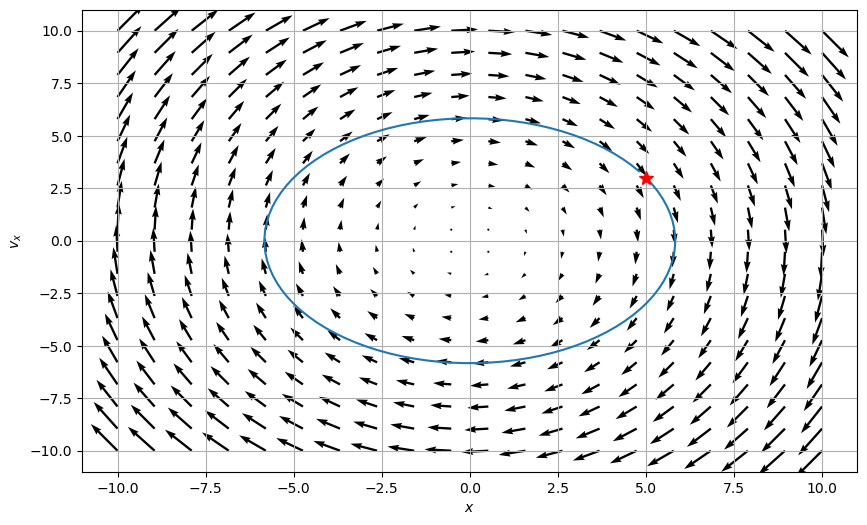
\includegraphics[keepaspectratio,alt={png}]{../images/notes-phase_space_notes-phase_space_tmp_18_0.png}}
\caption{png}
\end{figure}

\subsubsection{What can phase space help us
do?}\label{what-can-phase-space-help-us-do}

Let's remember a few things about the SHO.

\begin{enumerate}
\def\labelenumi{\arabic{enumi}.}
\tightlist
\item
  List all the things you know about the SHO. Include anything we
  haven't discussed (e.g., the energetics of the problem).
\item
  Name which of those things you can see in the phase diagram. Which
  things are you sure you can see? What things don't seem to be able to
  be seen from the phase diagram?
\item
  What do you remember about the energy of an SHO? Consider a harmonic
  oscillator in a known trajectory (\(x(t) = A\cos(\omega t)\)). Compute
  the total (conserved) energy of the oscillator as a function of time.

  \begin{itemize}
  \tightlist
  \item
    Explain how your expression for energy conservation can be seen in
    your phase diagram.
  \item
    You might try to show analytically that the ellipse above is related
    to your energy conservation expression
  \end{itemize}
\end{enumerate}

What does this plots tell you about all potential solutions?

\subsection{Handwritten Notes}\label{handwritten-notes}

Below, I have worked up some additional notes that describe the
conceptual and procedural aspects of phase space with respect to the
SHO.

\begin{itemize}
\tightlist
\item
  \href{../../assets/notes/Notes-Phase_Space.pdf}{Phase Space and the
  SHO}
\end{itemize}
